\documentclass[annual]{acmsiggraph}
%
\usepackage{graphicx}
\usepackage{pxfonts}
\usepackage{algorithm}
\usepackage{algorithmic}
\usepackage{epstopdf}
\usepackage{fullpage}
\usepackage{epic}
\usepackage{eepic}


\title{CS5625 Final Project: Nuts}

\author{Michael Flashman\thanks{e-mail:mtf53@cornell.edu}\\Cornell University \and Tianhe Zhang \thanks{e-mail:tz249@cornell.edu}\\Cornell University}

\pdfauthor{Michael Flashman, Tianhe Zhang}

\begin{document}


\maketitle


\section{The Goal}
An interactive palm tree in a wind-swept  desert, and balls.

\section{What did we achieve}
We procedurally generate  simple interactive palm trees.  The tree's various components, ie trunk, fronds, leaves are meshed using an underlying skeleton.  The skeleton is itself  wired to a physics engine as a mass and spring system.  Rather than build the complexity of the tree fully into the mesh or skeleton, we rely on the physics (and a dash of noise) to give each tree a unique appearance and  behavior.   This physics based approach further allows us to interact with the tree in interesting ways in the scene.   For instance, we can drop balls on our tree, or use the tree to  catapult the balls around our scene.  Tree modeling is fine, but to make life more interesting, we create a fully dynamic dessert scene, with moving sand dune and full day lighting.       

\section{What are the resources}

What we got off the Web or from other sources? Most of the algorithms/approaches used in our project come directly or indirectly from the technical papers and graphics related websites referenced below. We also found the course textbook to be useful from time to time. We developed our physics engine out of  a  2D particle simulation project for CS5643. The remainder of the project was developed and implemented by us.    

\section{What did we actually implement}
Below is a list of everything we did for this project, in chronological order.
\begin{itemize}
\item{Base code setup.}
\item{Extend physics engine to work in 3D.}
\item{Wire the physics engine to scene objects and associated mesh control points.} 
\item{Procedurally generate the trunk, fronds and leaves of the palm tree.}
\item{Extend Catmull--Clark subdivision surfaces to handle normals and texture coordinates.}
\item{Penalty forces as a proxy for  collision detection and resolution.}
\item{GPU based sand dune simulation and associated vertex displacement.}
\item{Normal/parallax mapping to bark textures (using only the diffuse texture map as input).}
\item{Dust/fog  layer to the sand dune.}
\item{Day light and Sky box implementation.}
\item{Game related implementation.}
\end{itemize}

Now for details on each of our components.
\begin{enumerate}
\item{\textbf{Base code}: We merge everything we have learned so far in the class so that the base code enables us to do shadow mapping, SSAO, subdivision surfaces and etc.}
\item{\textbf{Physics}: Skeleton of the tree represented by the particles and spring forces. The base code is from CS5643 but we modified several different forces such as bending and spring forces to make it work better for our model.}
\item{\textbf{Tree generation}: Procedurally generate the trunk, fronds and leaves of the palm tree. Using the skeleton particles (control points) to generate the mesh at run time. We applied the same model for the trunk and fronds. The skeleton of the trunk and fronds is a string of control particles. We use their positions to find the normals and binormals (same trick used for finding normals for bezier curve from last semester). The normals and binormals enable us to find 4 symmetric points around the each control particle.Connecting them gives us a cylinder mesh. We then use subdivision surface to make the mesh smoother. For the leaves, we use three control particles as the skeleton of the leave (as the middle stem). We added two additional points into the mesh so that the leaf has width. Then, we use subdivision surface to make the leave smoother on the edge.}
\item{\textbf{Expanded subdivision surfaces}: implemented normals and texture. Basically just interpolating values.}
\item{\textbf{Penalty forces}: is a way to handle collision easily. Set up a penalty distance. Whenever two particles are close (the distance is smaller the penalty distance), the force is applied to the particles to push them apart.}
\item{\textbf{Sand dune}: Our sand dune simulation is based on a model described in  \cite{momiji2002}.  This model captures granular transport phenomena due to wind shear, dune shadowing, and avalanche.  The primary challenge of our GPU implementation is handling long range transport phenomenon.  While cpu simulation has arbitrary read and write access to  data storage, on the GPU we can only write data to the current fragment location.  Instead, we rephrase the simulation as two stage stochastic process.  In the first stage, sand grains are released from each site with some probability  and placed in a special transport channel.  (Specifically, we store sand height in the r component of the gBuffer, and the transport grains in the g component of the gBuffer.)  One next pass each fragment samples its' neighbors to see if any grains are arriving, and accept them with some probability, and otherwise puts them back in the transport channel at the new location.    }
\item{\textbf{Parallax mapping}: To make our bark looks more realistic, we implemented parallax mapping which enables self shadowing according to the height map. The basic algorithm can be found from the textbook. We also implemented our own algorithm to find height map and normal map directly from the diffuse texture. The idea is easy: the brighter the pixel, the larger the height value. Normal map can then be found from the height map by looking around a pixel's surrounding values.}
\item{\textbf{Fog}: A windy sand dune should have some sand in the air. To that end we implement a height based fog model. The basic idea is described in \cite{hoffman2008}. Using the depth buffer as an indicator of fog density. We also implemented our own idea about the fog so that it only has fogging effect for at certain height. The idea is that transform points back to world space and compare the y value with the threshhold.  To give a more varied appearance,  we weight }
\item{\textbf{Day light and Sky box}: The basic idea is from http://www.henrybraun.info/skyrendering.html. We also implemented a simple sun model using linear/gaussian blur/interpolation.}
\item{\textbf{Game related}: Adding control and playability. }
\end{enumerate}

\section{What didn't we implement}
We implemented everything we promised in the proposal....more or less.   We struggled to do good procedural palm tree modeling, and our final results are obviously far from perfect.    It turns out that generating good vegetation is hard, and doing it in a way that allows for physical simulation is even harder.  In our proposal we also discussed procedural wind generation on the GPU.  It turn out to be much simpler to just add a wind force to the physics model,  similar to how gravity is implemented.  Finally we did not do procedural bark generation on the GPU.  While the fracture model would have been interesting, we instead focused on the GPU sand dune simulation  


\section{What we learned}
\begin{enumerate}
\item{\textbf{What was the best thing(s) you learned?} Making a computer game is fun. We have a much better understanding about multi-pass rendering in general, and glsl implementation specifically.   (especially debugging glsl) after this project.}
\item{\textbf{What were the gotchas?} In real time rending, actual physics doesn't matter. What matters is how it looks. Our way of modeling the palm tree is not as good as we expect and it takes longer time to configure. If we redo the project, we will choose other way to model and mesh the tree.}
\end{enumerate}

\section{What Effort We Make}
\begin{enumerate}
\item{Both of us work till the last minute.}
\item{Schedule}: We basically follow the timeline and work division in the proposal. The last two weeks we work together to make our game sharp. 
\end{enumerate}

\nocite{*}
\bibliographystyle{acmsiggraph}
\bibliography{bibliography}

\begin{figure*}
\begin{center}
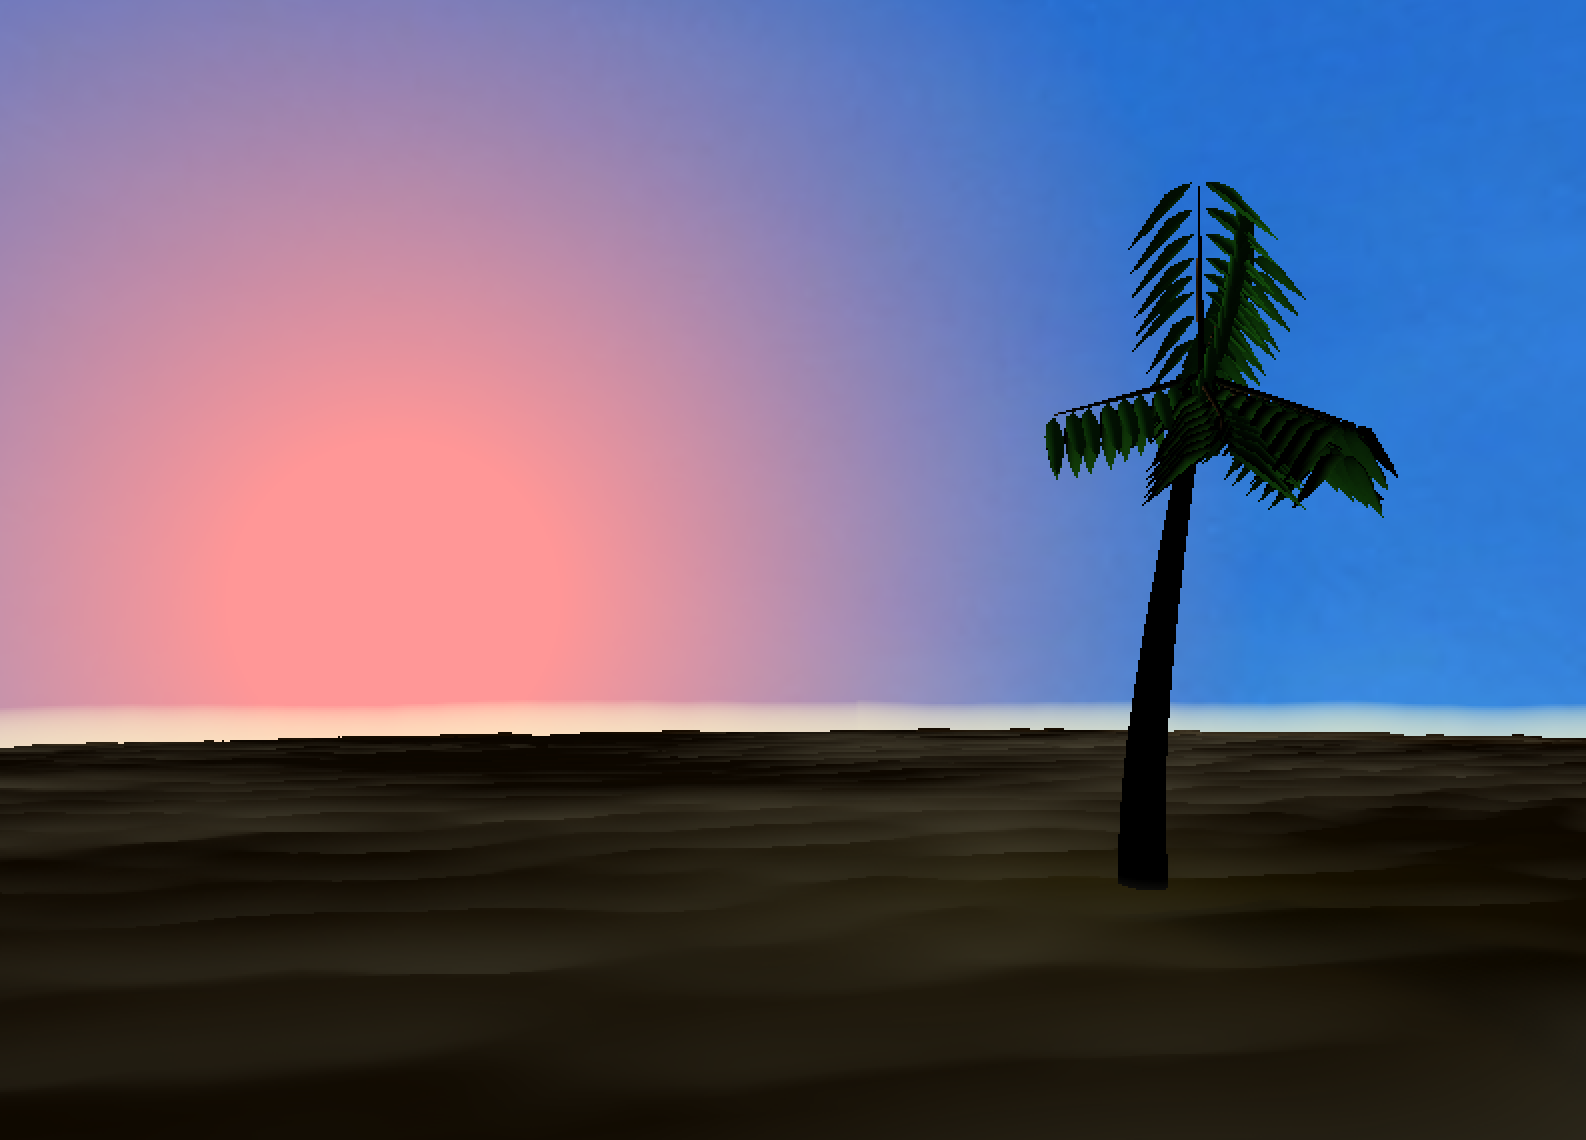
\includegraphics[width=500pt, height = 250pt]{fig1.png}
\caption{Screen shot during sun set.}
\end{center}
\end{figure*}

\begin{figure*}
\begin{center}
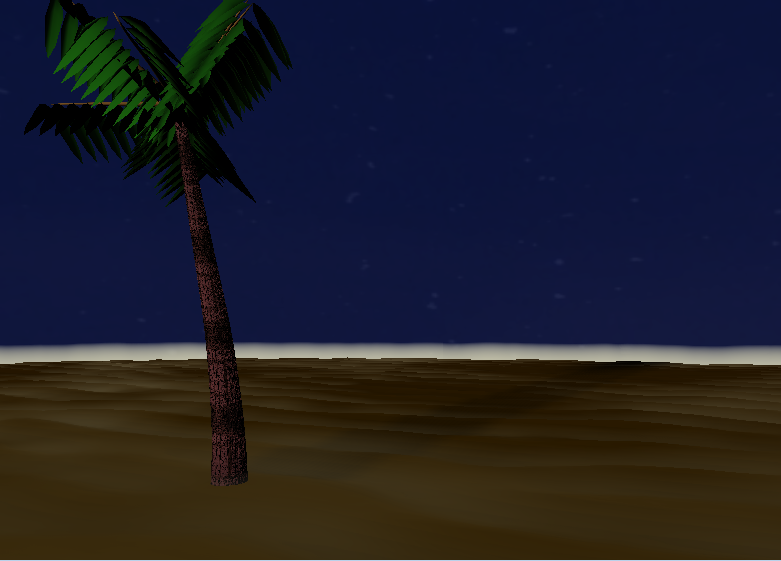
\includegraphics[width=500pt, height = 250pt]{fig2.png}
\caption{Screen shot during night.}
\end{center}
\end{figure*}

\begin{figure*}
\begin{center}
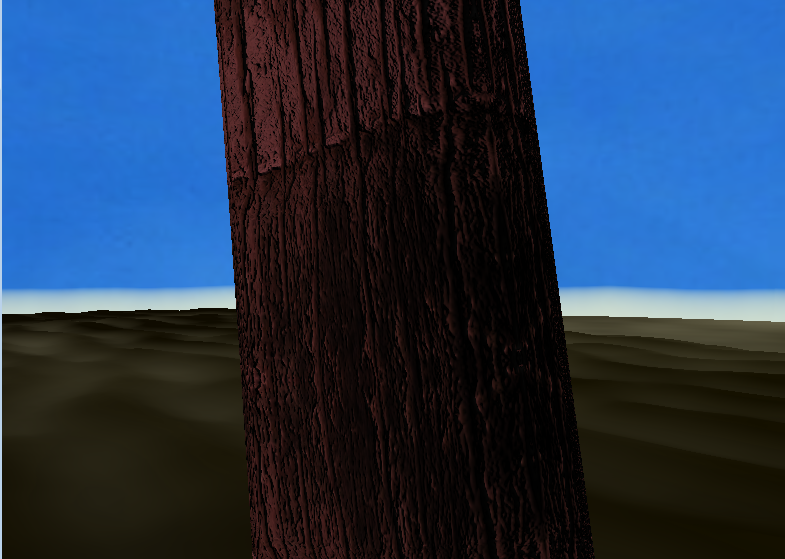
\includegraphics[width=500pt, height = 250pt]{fig3.png}
\caption{Close look at the parallax bark.}
\end{center}
\end{figure*}

\begin{figure*}
\begin{center}
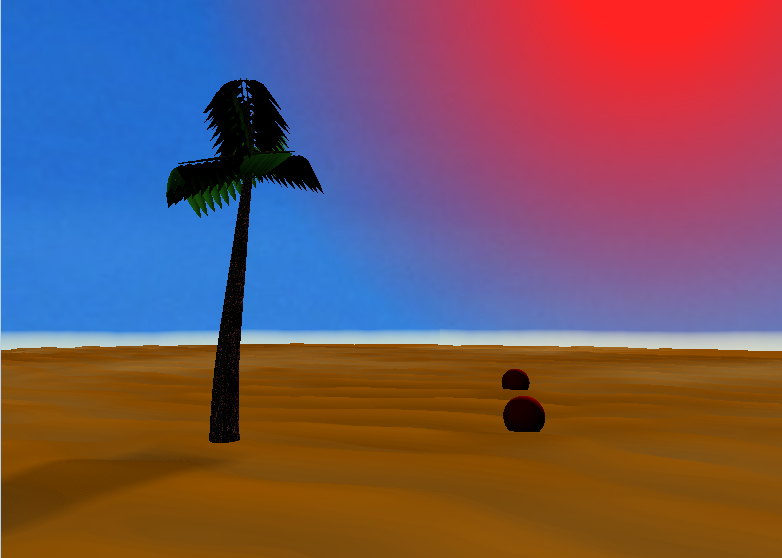
\includegraphics[width=500pt, height = 250pt]{fig4.png}
\caption{Tree interacts with the balls (cannot really see rom the photo).}
\end{center}
\end{figure*}

\end{document}
